\section{Uncomputing and Recomputing}
\subsection{Tock}

The key insight of Zombie is to introduce an abstraction layer between the executing program and the heap. This abstraction layer will allow the heap to transparently discard and recompute the program's intermediate values. To do so, we use the CEK machine to refer to each intermediate value by the index of the computation step that created it. Since each CEK step allocates at most one cell, this correspondence is injective. In other words, instead of storing pointers that refer to memory locations, we will store pointers, which we call ``tocks'', that refer to points in time---that is, CEK step indices.

In our runtime, these ``tocks'' are implemented as 64-bit integers, though in our model we will treat them as logically unbounded integers. There is a global ``current tock'' counter, which starts at 0 and is increased by 1 at every transition step in the abstract machine and at every allocation. The cell allocated at step $i$ is then referred to by the tock $i$, and that tock can then be used as a pointer, stored in data structures, looked up by later computations steps, and the like.

Note that, due to the determinism and linearity of the CEK machine, tocks are strictly ordered and the value computed at some tock $i$ can only depend on values computed at earlier tocks. Moreover we can recreate the value at tock $i$ by merely rerunning the CEK machine from some earlier state to that point. Because the CEK machine is deterministic, this re-execution will produce the same exact value as the original. Because our pointers refer to abstract values, not to specific memory locations, the heap can thus re-compute a value as necessary instead of storing it in memory.

In other words, the way Zombie works is that the heap will store only some of the intermediate values. The ones that aren't stored will instead be recomputed as needed, and the heap will store earlier CEK machine states in order to facilitate that. As the program runs, intermediate values can be discarded from the heap to reduce its memory usage.

Because a value can be recomputed from \emph{any} earlier CEK machine state, it will also turn out to be possible to store relatively few machine states. Therefore, overall memory usage---for the stored intermediate values and the stored machine states---can be kept low. In Zombie, we can store asymptotically fewer machine states than intermediate values, allowing us to asymptotically reduce memory usage.

\subsection{Tock Tree}

In Zombie, the heap is implemented by a runtime data structure called the tock tree. The tock tree maps tocks to the cells allocated by that step; in other words, the tock tree implements the mapping between tocks and their actual memory locations. Because values can be evicted to save memory, however, not all tocks have a mapping in the tock tree. Instead, every tock that \emph{is} present in the tock tree will also store its machine state. To recompute an evicted value at some tock $i$, the tock tree will find the largest machine state at tock $j < i$ and replay from that tock to tock $i$.

Each node in the Tock Tree stores both a memory cell and a machine state. Specifically, consider the execution of the CEK machine from step $t$. In step $t + 1$ it allocates a cell; it then performs a computation in step $t + 2$. So the node at tock $t$ contains both the cell allocated at step $t + 1$ as well as the machine state \emph{afterwards}, at step $t + 2$.

In order to make this operation efficient, the tock tree is organized as a binary search tree. In a binary search tree, arbitrary keys (tocks) can be looked up in $O(\log(n))$ time, where $n$ is the size of the tock tree, and when a key is not found, the largest key smaller than it can be easily found. Then the heap can replay execution from that point to compute the desired tock.

\begin{figure}
	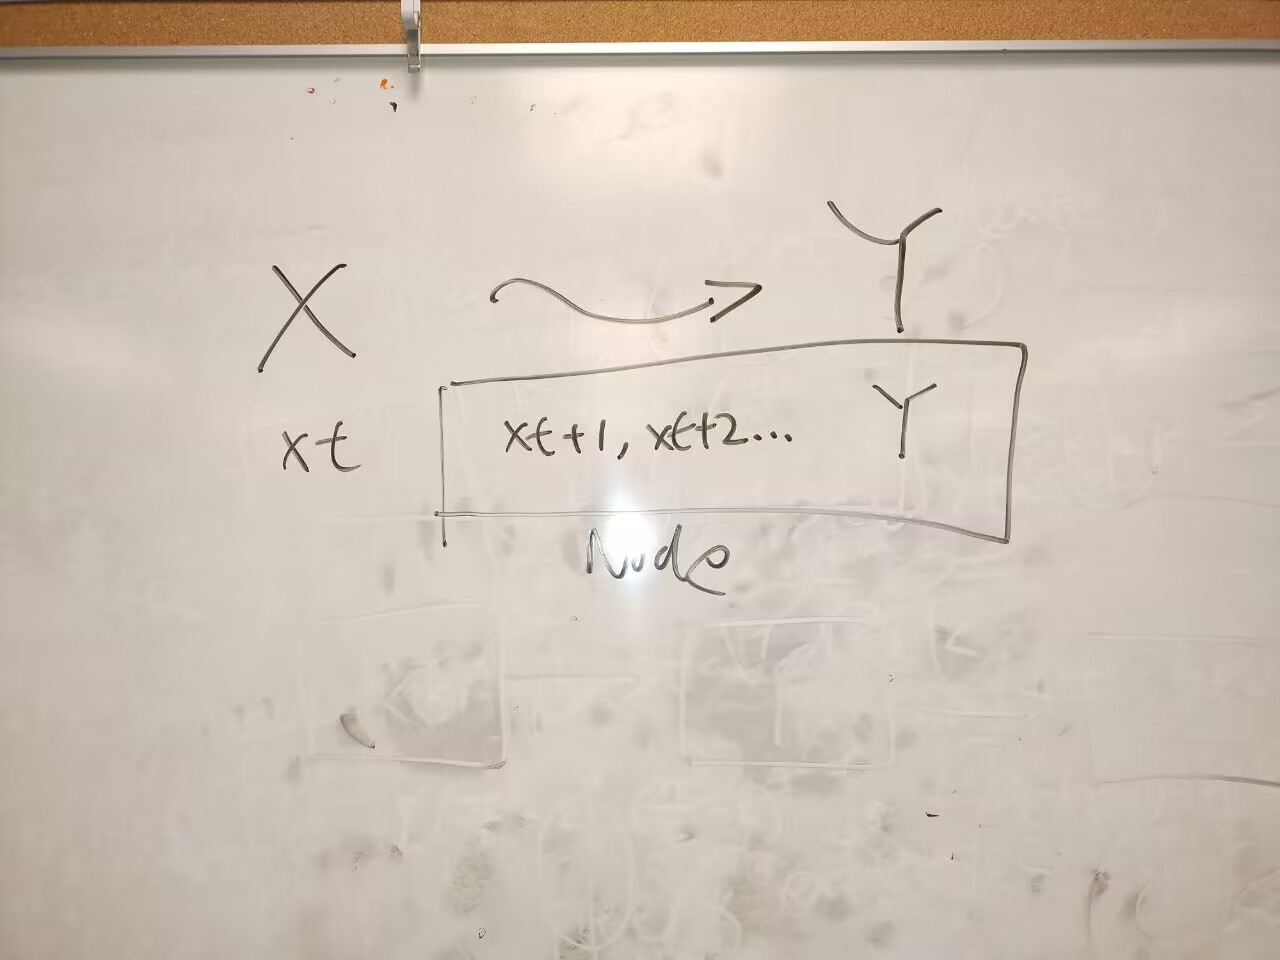
\includegraphics[width=0.5\columnwidth]{2}
	\caption{a node in the tock tree}
\end{figure}
\begin{figure}
	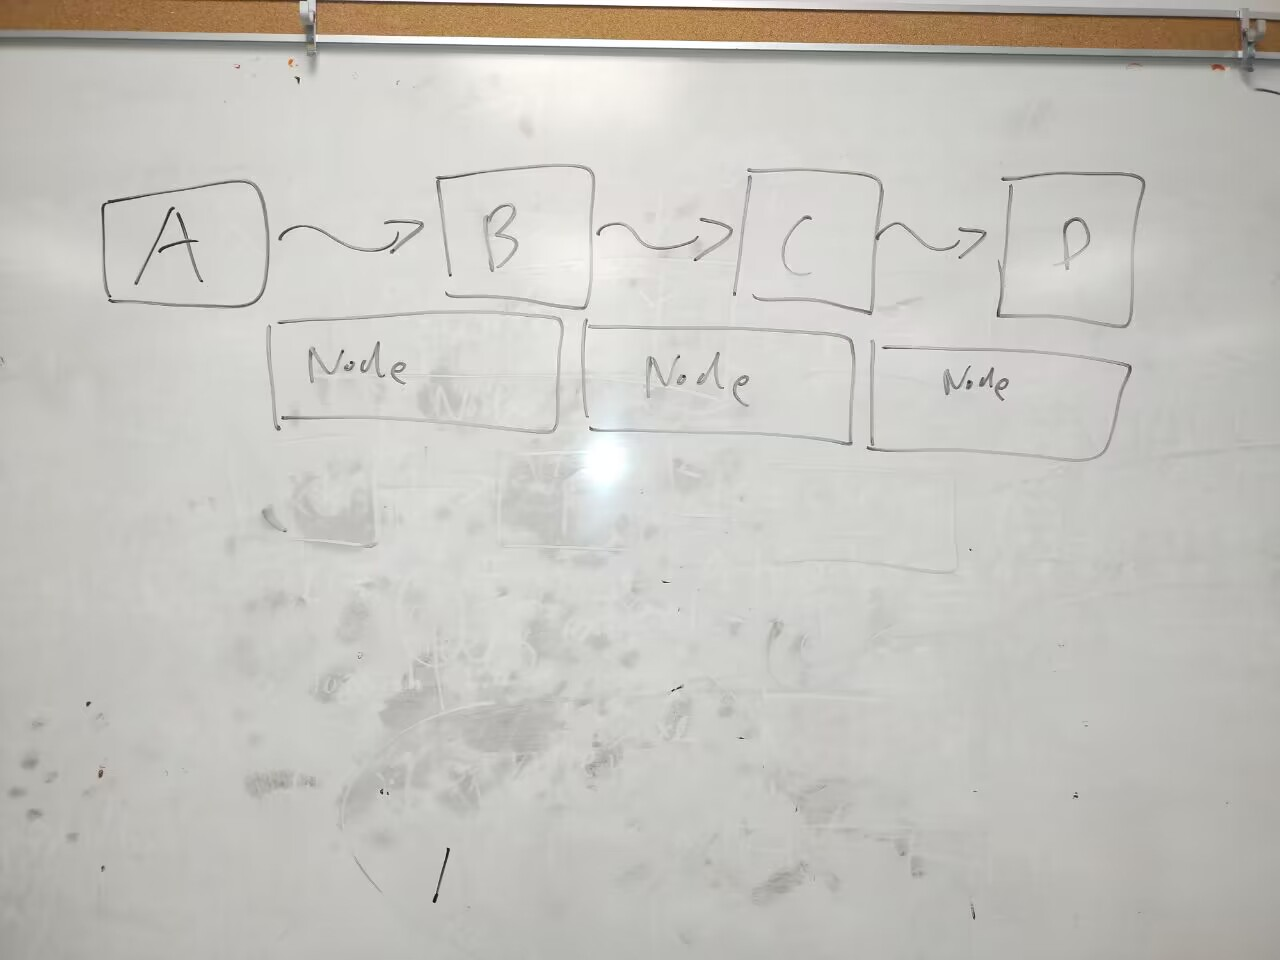
\includegraphics[width=0.5\columnwidth]{3}
	\caption{the tock tree with multiple nodes}
\end{figure}

\begin{figure}
	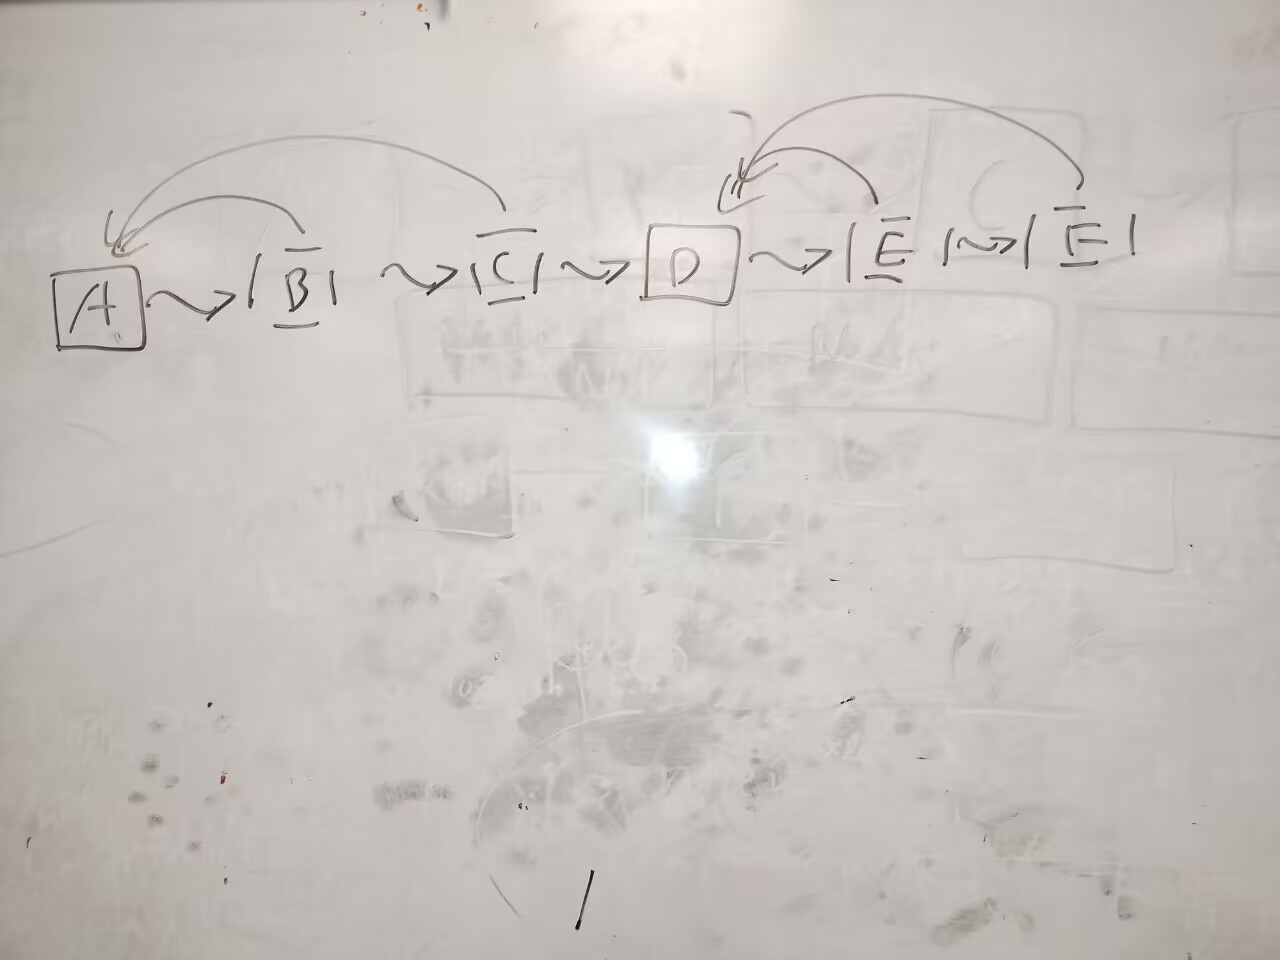
\includegraphics[width=0.5\columnwidth]{4}
	\caption{lookup failure return the latest earlier node}
\end{figure}


\subsection{Happy path}
Every state transition and pointer lookup is then converted into node insertion and node lookup into this data structure. After we had completed a transition, we construct the node, packing the allocated cells during the transition and the transit-to state, inserting the node onto the tock tree.

Originally, transition might require pointers lookup. Such lookup is translated to a query to the tock tree with the given node. Ideally speaking, the returned node contain the cell that correspond to the given tock. We can then convert the tock into the corresponding cell and continue execution. Note that we still need the tock tree to be lenient in this case, as the key of the node denote the beginning of the transition, not the cell itself.
\subsection{Sad Path}
Sadly, as we had removed nodes from the Tock Tree, we might not be able to retrieve a cell directly, and might need to recompute it - the point of the paper.

To recompute a value at tock t, the following steps are taken:
\begin{enumerate}
	\item Suspend the current execution into another kind of continuation, Replay Continuation (RK).
	\item Execute the transit-to state from the lookuped node in the tock tree, until tock reach t.
	\item Resume RK with the cell created at tock t.
\end{enumerate}
Note that the Replay Continuation operate at a more fine-grain granularity then that of the normal continuation. This is because a single transit step might do multiple lookup, but RK need to correspond to a lookup failure in such a transition. Otherwise the requested value might be immediately uncomputed again, and the whole process enter an infinite loop.

After the above 3 steps, the execution shall continue as if no replay had happens at all, and lookup return a node with the cell we wanted. In other words, the happy path and the sad path should converge.

During the replaying process, more lookup might be issued, and those lookup might need more replay - replay is recursive. Just like the classical continuation at the CEK machine, the Replay Continuation need to be recursive, and form a stack as well.

\subsection{Reified Continuation}
We treat continuations also as values, and label them with tock/put them in the tock tree, just like any other values. This allow us to also uncompute continuation as well.

\subsection{Eviction}

This allow us to remove any non-leftmost node from the tock tree. After the removal, the query that originally return the removed node, will return the node slightly earlier then that, which we can then replay to regenerate the removed node. In fact, this is the implementation of uncomputation in our system, and any non-leftmost node can be removed, to save memory at any given time.